\documentclass[11pt,a4paper]{article}

% ============================================================
% PACKAGES
% ============================================================
\usepackage[utf8]{inputenc}
\usepackage[T1]{fontenc}
\usepackage{amsmath,amssymb,amsthm}
\usepackage{mathtools}
\usepackage{physics}
\usepackage{geometry}
\usepackage{graphicx}
\usepackage{hyperref}
\usepackage{cleveref}
\usepackage{booktabs}
\usepackage{enumitem}
\usepackage{caption}
\usepackage{subcaption}
\usepackage{xcolor}
\usepackage{natbib}
\usepackage{fancyhdr}
\usepackage{titlesec}
\usepackage{appendix}
\usepackage{tikz}
\usetikzlibrary{shapes.geometric,arrows.meta,positioning,decorations.pathmorphing,calc,patterns,shadings}

% ============================================================
% GEOMETRY AND FORMATTING
% ============================================================
\geometry{margin=1in}
\setlength{\parskip}{0.5em}
\setlength{\parindent}{0pt}

% ============================================================
% THEOREM ENVIRONMENTS
% ============================================================
\newtheorem{definition}{Definition}[section]
\newtheorem{proposition}{Proposition}[section]
\newtheorem{theorem}{Theorem}[section]
\newtheorem{lemma}{Lemma}[section]
\newtheorem{remark}{Remark}[section]
\newtheorem{assumption}{Assumption}[section]

% ============================================================
% CUSTOM COMMANDS
% ============================================================
\newcommand{\phigr}{\varphi}
\newcommand{\defeq}{\coloneqq}
\newcommand{\Riem}{\mathcal{R}}
\newcommand{\Mani}{\mathcal{M}}
\newcommand{\Ent}{\mathcal{S}}
\newcommand{\Defect}{\mathcal{D}}
\newcommand{\Lapl}{\Delta}
\newcommand{\LaplB}{\Delta_{\text{LB}}}

% ============================================================
% HEADER AND FOOTER
% ============================================================
\pagestyle{fancy}
\fancyhf{}
\fancyhead[L]{\small Bridge Paper 3}
\fancyhead[R]{\small L.\ Smart}
\fancyfoot[C]{\thepage}
\renewcommand{\headrulewidth}{0.4pt}

% ============================================================
% TITLE INFORMATION
% ============================================================
\title{%
\textbf{Bridge Paper 3: Gravity from Geometric Non-Closure}\\[0.5em]
\large A $\phigr$-Scaled Scalar-Attractor Framework for Curvature, Entropy, and the Arrow of Time%
}

\author{%
Lee Smart\\[0.3em]
\textit{Vibrational Field Dynamics Institute}\\[0.3em]
\small Email: \href{mailto:contact@vibrationalfielddynamics.org}{contact@vibrationalfielddynamics.org}\\
\small X (Twitter): \href{https://twitter.com/vfd_org}{@vfd\_org}%
}

\date{December 4, 2025}

% ============================================================
% BEGIN DOCUMENT
% ============================================================
\begin{document}

\maketitle

\begin{center}
\textit{This paper is the third in a sequence of Bridge Papers developing the Vibrational Field Dynamics (VFD) framework.}
\end{center}

\vspace{1em}

% ============================================================
% ABSTRACT
% ============================================================
\begin{abstract}
This paper introduces geometric non-closure as a foundational mechanism from which spacetime curvature emerges as an effective response. Beginning with maximally symmetric local configurations---exemplified by the 120-cell as an archetype of perfect local closure---we demonstrate that global extension under expansion necessarily induces defect accumulation, quantified by a non-closure density field. The contraction dynamics and entropy monotonicity results established in Bridge Paper~2 are lifted from discrete graph structures to continuum manifolds via a correspondence between the $\phigr$-scaled graph Laplacian and the Laplace--Beltrami operator, where $\phigr = (1 + \sqrt{5})/2$ denotes the golden ratio. This lift yields a configurational entropy functional whose monotonic increase under geometric flow defines an intrinsic arrow of time without appeal to thermodynamic or cosmological boundary conditions. Gravity is then interpreted as the curvature response to accumulated geometric defects, yielding field equations compatible with the Einstein equations in appropriate limits, supplemented by a defect-induced stress-energy contribution. The framework offers falsifiable predictions amenable to discrete simulations, continuum modelling, and analogues in condensed-matter systems.
\end{abstract}

\vspace{1em}

% ============================================================
% KEY CONTRIBUTIONS
% ============================================================
\section*{Key Contributions}

\begin{itemize}[leftmargin=2em]
\item \textbf{Geometric Non-Closure as Defect Density:} We provide a precise definition of non-closure arising from the impossibility of globally extending maximally symmetric local configurations, and encode this as a scalar defect density field $\Defect(x)$.

\item \textbf{Continuum Lift of BP2 Contraction:} The discrete $\phigr$-scaled contraction dynamics and spectral decay results of Bridge Paper~2 are systematically lifted to a continuum entropy functional on Riemannian manifolds via the Laplace--Beltrami correspondence.

\item \textbf{Einstein-Compatible Effective Curvature Response:} We derive an effective action whose variation yields field equations of Einstein form, with the defect density contributing an additional geometric stress-energy term that modifies the standard vacuum equations.

\item \textbf{Arrow of Time from Geometric Dephasing:} The monotonic increase of the configurational entropy functional under $\phigr$-scaled flow establishes a geometric arrow of time, identified with irreversible accumulation of phase defects rather than thermodynamic assumptions.

\item \textbf{Falsifiable Predictions and Simulation Pathways:} We present a structured set of predictions specifying observable signatures, expected scalings, and falsification criteria, together with concrete pathways for discrete simulation and continuum modelling.
\end{itemize}

\vspace{1em}

% ============================================================
% SECTION 1: MOTIVATION AND NARRATIVE HINGE
% ============================================================
\section{Motivation and Narrative Hinge}
\label{sec:motivation}

The progression from Bridge Paper~1 (BP1) through Bridge Paper~2 (BP2) established a discrete geometric framework in which $\phigr$-scaled dynamics govern spectral contraction and entropy evolution on graph structures \citep{BP2}. A natural question arises: what role does gravity play within this framework, and how does spacetime curvature relate to the geometric mechanisms already developed?

This paper addresses that question, but does so with deliberate restraint. Before introducing gravitational dynamics, it is essential to clarify the geometric substrate upon which such dynamics might operate. Specifically, we must understand why \emph{maximal local symmetry}---the condition of perfect geometric closure at each vertex or cell---cannot be maintained under global extension.

\subsection{Why Maximal Symmetry Precedes Gravity}

The standard approach to gravity begins with a smooth manifold equipped with a metric and proceeds to the Einstein equations via variational principles. Our approach inverts this logic: we begin with a discrete, combinatorially defined notion of local closure and ask what constraints arise when such closure is demanded globally.

The answer, as we shall demonstrate, is that perfect global closure is generically impossible. The obstruction is not dynamical but purely geometric: the angular and combinatorial constraints that permit local closure become mutually incompatible upon iteration. This incompatibility manifests as \emph{defects}---irreducible deviations from the locally closed ideal that accumulate under expansion.

Once defects are recognised as inevitable, gravity emerges not as a fundamental force but as the effective curvature response to defect accumulation. This reframing places geometric structure logically prior to gravitational dynamics.

\subsection{The 120-Cell as Archetype}

Throughout this paper, we employ the 120-cell---the regular 4-polytope with 120 dodecahedral cells meeting at 600 vertices---as an archetype of maximal local closure in four dimensions. This choice is made for concreteness, not exclusivity.

The 120-cell is the unique regular 4-polytope that achieves maximal vertex valence and cell count among the six regular 4-polytopes. Its structure exemplifies the principle that local closure, when pushed to its symmetric limit, admits no global iteration without defect.

We emphasise that the 120-cell serves as a \emph{representative example} of a general principle. The results of this paper do not depend on the literal tiling of spacetime by 120-cells, nor do we claim that physical spacetime possesses such a structure. Rather, the 120-cell illustrates the geometric obstruction that any maximally symmetric local configuration must confront upon extension.

\subsection{What This Paper Does Not Claim}
\label{subsec:disclaimers}

To prevent misinterpretation, we state explicitly what this paper does \emph{not} claim:

\begin{itemize}[leftmargin=2em]
\item \textbf{No replacement of General Relativity:} The effective field equations derived here are compatible with the Einstein equations in appropriate limits. We do not claim to supersede or contradict General Relativity; rather, we offer a geometric interpretation of its structure.

\item \textbf{No new forces or particles:} Gravity is interpreted as an emergent curvature response, not as a new fundamental interaction. No new particles, fields beyond those already present, or modifications to the Standard Model are introduced.

\item \textbf{No cosmological speculation:} We do not address the origin of the universe, the nature of dark energy, or inflationary dynamics. The scope is limited to the emergence of effective curvature from geometric non-closure.

\item \textbf{No consciousness or metaphysical claims:} The arrow of time derived here is purely geometric, defined by functional monotonicity. No claims about the nature of consciousness, free will, or the metaphysics of time are made or implied.

\item \textbf{No claim of completeness:} This framework is presented as a candidate explanatory structure, not a finished theory. Known limitations are discussed in Section~\ref{sec:discussion}.
\end{itemize}

\subsection{The Abstraction, Not the Leap}

Bridge Paper~3 occupies a specific position in the sequence: it \emph{abstracts} from the discrete results of BP2 to continuum geometry, and it \emph{identifies} the mechanism by which curvature might emerge from defects. It does not leap to a full gravitational theory, nor does it claim to derive General Relativity from first principles.

The progression is:
\begin{enumerate}
\item BP2 established $\phigr$-scaled contraction and entropy monotonicity on discrete graphs.
\item BP3 lifts these results to continuum manifolds and identifies defects as the geometric origin of curvature.
\item Future work will explore the dynamical consequences, cosmological implications, and quantitative predictions in greater detail.
\end{enumerate}

This paper completes the second step.

% ============================================================
% SECTION 2: GEOMETRIC SUBSTRATE
% ============================================================
\section{Geometric Substrate: Closure, Extension, and Non-Closure}
\label{sec:substrate}

We now develop the geometric foundations upon which the remainder of the paper rests. The key concepts are \emph{local closure}, \emph{global extension}, and \emph{non-closure} (defect density).

\subsection{Definitions}
\label{subsec:definitions}

\begin{definition}[Cell Complex]
A \emph{cell complex} $\mathcal{K}$ is a topological space constructed by iteratively attaching cells of increasing dimension: 0-cells (vertices), 1-cells (edges), 2-cells (faces), and so forth. We denote the set of $k$-cells by $\mathcal{K}^{(k)}$.
\end{definition}

\begin{definition}[Local Closure]
A cell complex $\mathcal{K}$ is \emph{locally closed at a vertex} $v \in \mathcal{K}^{(0)}$ if the link of $v$---the boundary of a small neighbourhood of $v$---is a closed manifold of appropriate dimension with no boundary or singularity.
\end{definition}

In dimension 4, local closure at a vertex requires the link to be a closed 3-manifold. For the 120-cell, the vertex link is a tetrahedron (the vertex figure), reflecting the local combinatorial structure.

\begin{definition}[Global Extension]
A locally closed complex $\mathcal{K}$ admits \emph{global extension} if it can be iteratively grown by attaching new cells while preserving local closure at every vertex.
\end{definition}

\begin{definition}[Defect / Non-Closure Density]
Let $\mathcal{K}$ be a cell complex that is locally closed except at a set of vertices $V_{\text{def}} \subset \mathcal{K}^{(0)}$. The \emph{defect density} at a point $x$ in a continuum limit is defined as
\begin{equation}
\Defect(x) \defeq \lim_{\epsilon \to 0} \frac{1}{\text{Vol}(B_\epsilon(x))} \sum_{v \in V_{\text{def}} \cap B_\epsilon(x)} \delta_v,
\label{eq:defect-density}
\end{equation}
where $B_\epsilon(x)$ is a ball of radius $\epsilon$ centred at $x$, and $\delta_v$ is the local angular or combinatorial deficit at vertex $v$.
\end{definition}

The defect density $\Defect(x)$ is a non-negative scalar field that vanishes where local closure is achieved and is positive where defects have accumulated.

\subsection{Maximal Local Closure: The 120-Cell}
\label{subsec:120cell}

The 120-cell is the four-dimensional regular polytope with Schläfli symbol $\{5, 3, 3\}$. Its structure is as follows:
\begin{itemize}
\item 600 vertices
\item 1200 edges
\item 720 pentagonal faces
\item 120 dodecahedral cells
\end{itemize}

Each vertex is shared by exactly 4 dodecahedral cells, and the vertex figure is a regular tetrahedron. The 120-cell achieves \emph{maximal local closure} in the sense that no regular 4-polytope has greater vertex valence or cell complexity.

The dimensional generality of this principle must be emphasised. In three dimensions, the analogous structure is the dodecahedron with icosahedral vertex links. In higher dimensions, analogous polytopes exist (the $n$-dimensional regular polytopes), though their enumeration becomes sparse. The \emph{principle}---that maximal local symmetry imposes constraints on global extension---transcends any particular dimension.

\subsection{Why Expansion Forces Non-Closure}
\label{subsec:expansion-nonclosure}

The central geometric observation of this section is:

\begin{proposition}[Obstruction to Global Extension]
\label{prop:obstruction}
Let $\mathcal{K}$ be a locally closed cell complex achieving maximal symmetry at each vertex (e.g., derived from a regular polytope). Then $\mathcal{K}$ cannot be globally extended to tile an unbounded region while preserving local closure at all vertices.
\end{proposition}

The proof, which we outline rather than present in full rigour, proceeds as follows:

\begin{enumerate}
\item \textbf{Dihedral angle constraints:} Local closure at each vertex imposes a constraint on the dihedral angles of the incident cells. For a regular polytope $\{p, q, r\}$, the dihedral angle $\theta$ of each cell is fixed by the Schläfli symbol.

\item \textbf{Coxeter honeycomb obstruction:} A regular polytope can tile Euclidean space if and only if an integer number of cells fit around each codimension-2 face, i.e., $2\pi / \theta \in \mathbb{Z}$ with $\theta$ in radians. The 120-cell $\{5, 3, 3\}$ is a \emph{spherical} polytope: its dihedral angle $\theta \approx 2.513\,\text{rad}$ ($\approx 144°$) does not divide $2\pi$ evenly. Consequently, the 120-cell cannot tile flat $\mathbb{R}^4$---it closes only on the 3-sphere $S^3$. This is a special case of the classification of regular honeycombs \citep{Coxeter1973}.

\item \textbf{Extension conflict:} Attempting to extend a 120-cell configuration in flat space forces either angular gaps (where fewer cells meet than required) or angular overlaps (where more cells meet). Both represent deviations from local closure.

\item \textbf{Defect accumulation:} To continue extension in flat space, one must either (a) introduce vertices where local closure fails (angular deficits or excesses), or (b) embed in curved space where the angular constraints can be satisfied. Both options correspond to the accumulation of defects or curvature.
\end{enumerate}

This obstruction is analogous to the impossibility of tiling a flat plane with regular pentagons: local closure (each tile meeting edge-to-edge) is achievable, but global extension inevitably introduces gaps or overlaps.

\begin{figure}[ht]
\centering
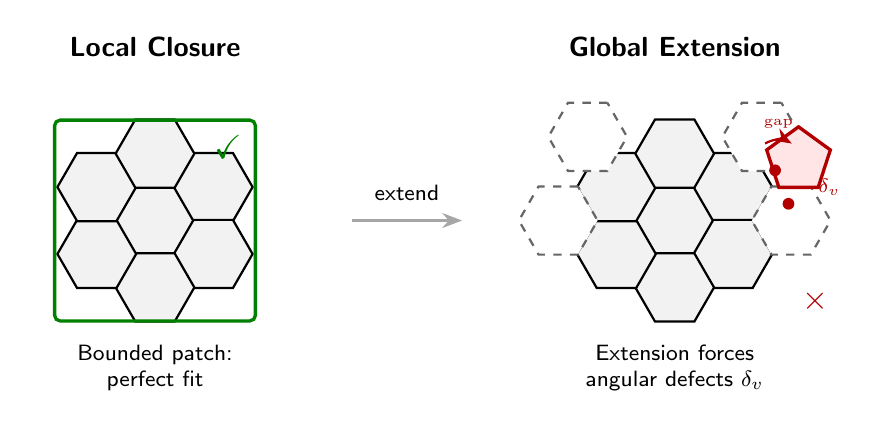
\begin{tikzpicture}[
    cell/.style={regular polygon, regular polygon sides=6, minimum size=1cm, draw=black, thick, fill=gray!10},
    defectcell/.style={regular polygon, regular polygon sides=6, minimum size=1cm, draw=black!60, thick, fill=white, dashed},
    gapcell/.style={regular polygon, regular polygon sides=5, minimum size=0.85cm, draw=red!70!black, very thick, fill=red!10},
    annotation/.style={font=\footnotesize\sffamily, align=center},
    arrow/.style={-{Stealth[length=2.5mm]}, thick, gray!70}
]
% LEFT PANEL: Local Closure
\begin{scope}[shift={(-3.8,0)}, scale=0.85]
    \node[annotation, font=\sffamily\bfseries] at (0,2.6) {Local Closure};
    \node[cell] (c0) at (0,0) {};
    \node[cell] (c1) at (0.87,0.5) {};
    \node[cell] (c2) at (0.87,-0.5) {};
    \node[cell] (c3) at (0,-1) {};
    \node[cell] (c4) at (-0.87,-0.5) {};
    \node[cell] (c5) at (-0.87,0.5) {};
    \node[cell] (c6) at (0,1) {};
    \draw[green!50!black, very thick, rounded corners=2pt] (-1.5,-1.5) rectangle (1.5,1.5);
    \node[green!50!black, font=\large] at (1.1,1.1) {\checkmark};
    \node[annotation, text width=3cm] at (0,-2.2) {Bounded patch:\\perfect fit};
\end{scope}
% ARROW
\draw[arrow, line width=1.2pt] (-1.3,0) -- (0.1,0);
\node[annotation] at (-0.6,0.35) {extend};
% RIGHT PANEL: Global Extension with Defects
\begin{scope}[shift={(2.8,0)}, scale=0.85]
    \node[annotation, font=\sffamily\bfseries] at (0,2.6) {Global Extension};
    \node[cell] (d0) at (0,0) {};
    \node[cell] (d1) at (0.87,0.5) {};
    \node[cell] (d2) at (0.87,-0.5) {};
    \node[cell] (d3) at (0,-1) {};
    \node[cell] (d4) at (-0.87,-0.5) {};
    \node[cell] (d5) at (-0.87,0.5) {};
    \node[cell] (d6) at (0,1) {};
    \node[defectcell] (e1) at (1.74,0) {};
    \node[defectcell] (e2) at (1.3,1.25) {};
    \node[defectcell] (e3) at (-1.3,1.25) {};
    \node[defectcell] (e4) at (-1.74,0) {};
    \node[gapcell] (gap1) at (1.85,0.9) {};
    \fill[red!70!black] (1.5,0.75) circle (2.5pt);
    \fill[red!70!black] (1.7,0.25) circle (2.5pt);
    \node[red!70!black, font=\scriptsize\bfseries, right] at (2.0,0.5) {$\delta_v$};
    \draw[red!70!black, thick, -{Stealth}] (1.35,1.15) arc (120:60:0.4);
    \node[red!70!black, font=\tiny] at (1.55,1.45) {gap};
    \node[red!70!black, font=\large] at (2.1,-1.2) {$\times$};
    \node[annotation, text width=3.2cm] at (0,-2.2) {Extension forces\\angular defects $\delta_v$};
\end{scope}
\end{tikzpicture}
\caption{Local closure versus global extension. \textit{Left:} A bounded patch of cells achieves perfect local closure at all vertices. \textit{Right:} Attempting global extension forces angular mismatches (defects $\delta_v$) at boundary vertices where dihedral angle constraints cannot be simultaneously satisfied.}
\label{fig:defect-accumulation}
\end{figure}

\subsection{Defects as Stored Geometric History}
\label{subsec:defects-history}

A crucial property of defects is their \emph{irreversibility}. Once a defect is introduced during extension, it cannot be removed by local rearrangements or coordinate transformations. This irreversibility has several important consequences:

\begin{itemize}
\item \textbf{Defects are physical:} Unlike coordinate artefacts, defects represent genuine obstructions to local closure. They are invariant under diffeomorphisms of the ambient space.

\item \textbf{Defects accumulate monotonically:} Under continued expansion, the total defect content can only increase (or remain constant). There is no mechanism for defect annihilation in the absence of topology change.

\item \textbf{Defects encode history:} The spatial distribution of defects reflects the sequence of extensions that produced the current configuration. In this sense, defects constitute a ``geometric memory'' of the complex's growth.
\end{itemize}

These properties will be essential in Section~\ref{sec:entropy}, where we connect defect accumulation to entropy monotonicity and the arrow of time.

% ============================================================
% SECTION 3: BP2 TO CONTINUUM ENTROPY
% ============================================================
\section{From BP2 Contraction to a Continuum Entropy Functional}
\label{sec:entropy}

This section constructs the bridge from the discrete results of BP2 to continuum geometry. The key step is the correspondence between the $\phigr$-scaled graph Laplacian and the Laplace--Beltrami operator on Riemannian manifolds.

\subsection{Summary of BP2 Results}
\label{subsec:bp2-summary}

Bridge Paper~2 \citep{BP2} established the following results for dynamics on discrete graph structures:

\begin{enumerate}
\item \textbf{$\phigr$-Scaled Contraction Law:} Let $G = (V, E)$ be a finite graph with adjacency matrix $A$ and degree matrix $D$. The graph Laplacian $L = D - A$ generates a diffusion process. Under $\phigr$-scaling, the contraction rate of probability distributions is governed by
\begin{equation}
\frac{d}{dt} \| \rho_t - \rho_\infty \|_2 \leq -\phigr \cdot \lambda_1 \| \rho_t - \rho_\infty \|_2,
\label{eq:bp2-contraction}
\end{equation}
where $\lambda_1 > 0$ is the spectral gap of $L$ and $\rho_\infty$ is the equilibrium distribution.

\item \textbf{Spectral Decay:} The eigenvalues of the time-evolution operator decay exponentially with rates proportional to $\phigr \lambda_k$, where $\lambda_k$ is the $k$-th eigenvalue of $L$.

\item \textbf{Entropy Monotonicity:} A discrete configurational entropy
\begin{equation}
S_{\text{disc}}[\rho] = -\sum_{v \in V} \rho(v) \log \rho(v)
\label{eq:discrete-entropy}
\end{equation}
increases monotonically under the $\phigr$-scaled flow until equilibrium is reached.
\end{enumerate}

These results apply to finite graphs with appropriate connectivity and spectral properties. The question now is: how do they generalise to continuum manifolds?

\subsection{Discrete to Continuum Lift}
\label{subsec:discrete-continuum}

The correspondence between discrete and continuum geometry is implemented via the following identifications:

\begin{itemize}
\item \textbf{Graph Laplacian $\to$ Laplace--Beltrami Operator:} The graph Laplacian $L$ acting on functions $f: V \to \mathbb{R}$ corresponds to the Laplace--Beltrami operator $\LaplB$ acting on functions $f: \Mani \to \mathbb{R}$ on a Riemannian manifold $(\Mani, g)$:
\begin{equation}
\LaplB f = \frac{1}{\sqrt{|g|}} \partial_\mu \left( \sqrt{|g|} g^{\mu\nu} \partial_\nu f \right).
\label{eq:laplace-beltrami}
\end{equation}

\item \textbf{Vertex Sums $\to$ Integrals:} Sums over vertices $\sum_{v \in V}$ become integrals over the manifold $\int_\Mani \sqrt{|g|} \, d^n x$.

\item \textbf{Edge Weights $\to$ Metric Coefficients:} Edge weights in a weighted graph correspond to components of the metric tensor $g_{\mu\nu}$.

\item \textbf{Defect Vertices $\to$ Defect Density Field:} The set of defect vertices $V_{\text{def}}$ lifts to the continuum defect density $\Defect(x)$ defined in Eq.~\eqref{eq:defect-density}.
\end{itemize}

These correspondences are well-established in spectral geometry and form the basis for numerical methods such as discrete exterior calculus and finite element analysis on manifolds \citep{Desbrun2005}.

\begin{assumption}[Regularity]
\label{ass:regularity}
The limiting manifold $(\Mani, g)$ is smooth, oriented, and complete. The defect density $\Defect(x)$ is bounded and integrable.
\end{assumption}

\begin{assumption}[Spectral Correspondence]
\label{ass:spectral}
The spectrum of the graph Laplacian $L$ on a sequence of refining graphs converges to the spectrum of $\LaplB$ on the limiting manifold.
\end{assumption}

Under these assumptions, the BP2 contraction law lifts to:
\begin{equation}
\frac{d}{dt} \| \rho_t - \rho_\infty \|_{L^2(\Mani)} \leq -\phigr \cdot \lambda_1^{(\text{LB})} \| \rho_t - \rho_\infty \|_{L^2(\Mani)},
\label{eq:continuum-contraction}
\end{equation}
where $\lambda_1^{(\text{LB})} > 0$ is the first nonzero eigenvalue of $\LaplB$.

\subsection{Configurational Entropy Functional}
\label{subsec:entropy-functional}

With the continuum lift in place, we define the configurational entropy functional:

\begin{definition}[Configurational Entropy]
\label{def:entropy}
Let $\rho: \Mani \to \mathbb{R}_{\geq 0}$ be a normalised density on $(\Mani, g)$. The \emph{configurational entropy} is
\begin{equation}
\Ent[\rho] \defeq -\int_\Mani \rho(x) \log \rho(x) \sqrt{|g|} \, d^n x.
\label{eq:entropy-functional}
\end{equation}
\end{definition}

This entropy measures the breadth of the accessible configuration space. It is distinct from thermodynamic entropy in that it depends only on the geometric distribution $\rho$, not on temperature, energy, or other thermodynamic variables.

Under the $\phigr$-scaled Laplace--Beltrami flow
\begin{equation}
\frac{\partial \rho}{\partial t} = \phigr \cdot \LaplB \rho,
\label{eq:phi-flow}
\end{equation}
the entropy functional satisfies:

\begin{proposition}[Entropy Increase]
\label{prop:entropy-increase}
Under the flow \eqref{eq:phi-flow}, the configurational entropy $\Ent[\rho_t]$ is non-decreasing:
\begin{equation}
\frac{d\Ent}{dt} = \phigr \int_\Mani \frac{|\nabla \rho|^2}{\rho} \sqrt{|g|} \, d^n x \geq 0.
\label{eq:entropy-increase}
\end{equation}
Equality holds if and only if $\rho$ is constant (the equilibrium state).
\end{proposition}

This result is the continuum analogue of the BP2 entropy monotonicity theorem. The quantity $\int |\nabla \rho|^2 / \rho$ is the Fisher information, and its positivity drives entropy increase.

\begin{remark}[Entropy Convention]
\label{rem:entropy-convention}
A potential source of confusion must be addressed. In BP2, the central result concerns \emph{spectral contraction}: the distance between an evolving distribution and equilibrium decreases monotonically. In the continuum setting, we speak of \emph{entropy increase}: the configurational entropy grows toward its maximum at equilibrium. These are dual descriptions of the same underlying geometric process. Contraction in distribution space (measured by $L^2$ or related norms) corresponds to expansion of the effective volume of accessible configurations (measured by entropy). Both quantities track relaxation toward equilibrium; they are related by $\Ent[\rho] \sim \log(\text{accessible configuration volume})$. Crucially, this entropy is configurational and geometric---it quantifies the spread of a distribution over the manifold and should not be conflated with thermodynamic entropy, which depends on temperature, energy, and microphysical degrees of freedom not present in this framework.
\end{remark}

\subsection{The Arrow of Time}
\label{subsec:arrow-time}

The monotonic increase of $\Ent[\rho_t]$ provides an intrinsic definition of the arrow of time within this framework:

\begin{definition}[Geometric Arrow of Time]
The \emph{arrow of time} is the direction along which $\Ent[\rho_t]$ increases (equivalently, the direction along which the defect density $\Defect$ accumulates).
\end{definition}

This definition has several notable features:

\begin{itemize}
\item \textbf{No thermodynamic assumption:} The arrow of time is defined geometrically, without reference to heat, temperature, or the second law of thermodynamics.

\item \textbf{No cosmological boundary condition:} Unlike approaches that derive the arrow of time from a low-entropy initial state of the universe, this definition is local and does not require global cosmological assumptions.

\item \textbf{Compatibility with microscopic reversibility:} The underlying dynamics (heat flow) are reversible; the arrow emerges from the choice of initial conditions, not from irreversibility of the fundamental law.
\end{itemize}

We emphasise that this is \emph{one} way to define an arrow of time, not a claim that it is the unique or fundamental definition. The relationship to thermodynamic and cosmological arrows remains an open question.

To summarise the geometric origin of temporal asymmetry: within this framework, the arrow of time arises from three interrelated mechanisms. First, the configurational entropy $\Ent[\rho]$ increases monotonically under geometric flow, providing a scalar measure that distinguishes past from future. Second, defect accumulation is irreversible---once geometric non-closure is introduced during extension, it cannot be undone by local operations, yielding a ratchet-like asymmetry. Third, the $\phigr$-scaled contraction dynamics drive loss of phase coherence as distributions relax toward equilibrium, erasing fine-grained geometric information. Together, these mechanisms establish an emergent, geometric arrow of time that does not depend on thermodynamic assumptions or cosmological boundary conditions. This structural origin of temporal asymmetry is consistent with relativistic causality: the monotonic functional $\Ent[\rho]$ respects the causal structure inherited from the continuum metric, ensuring that the geometric arrow aligns with the light-cone structure of the effective spacetime.

% ============================================================
% SECTION 4: GRAVITY AS EMERGENT CURVATURE
% ============================================================
\section{Gravity as Emergent Curvature Response}
\label{sec:gravity}

We now arrive at the central claim of this paper: gravity emerges as the effective curvature response to accumulated geometric defects.

Before proceeding, we state explicitly the ontological status of gravity within this framework. Gravity is \emph{not} treated here as a fundamental interaction in the sense of a primary force mediating between matter sources. Rather, gravity appears as an \emph{emergent} phenomenon: it is the effective geometric response that arises when the accumulation of non-closure defects is described in a continuum approximation. Einstein gravity---the dynamics encoded in the Einstein field equations---emerges as the leading-order continuum limit of this underlying discrete geometry. In this sense, curvature acts as geometric bookkeeping for defect density: regions of high defect accumulation correspond, in the effective description, to regions of nonzero curvature. No new fundamental force is introduced; instead, what we conventionally call ``gravitational dynamics'' is reinterpreted as the continuum manifestation of geometric constraints that cannot be satisfied under global extension.

\subsection{Geometry as Bookkeeping}
\label{subsec:bookkeeping}

The perspective we adopt is that \emph{curvature is bookkeeping for defects}. When local closure fails, the deviation from flatness must be recorded somewhere. In the discrete setting, this is recorded at defect vertices. In the continuum, it is encoded in the curvature tensor.

This perspective is not new. Regge calculus \citep{Regge1961} discretises General Relativity by concentrating curvature at the hinges (codimension-2 simplices) of a simplicial complex. Our approach is similar in spirit but differs in starting point: we begin with maximal local closure and derive defects from extension failure, rather than starting with a simplicial approximation to a smooth manifold.

The key identification, in an effective continuum description, is:
\begin{equation}
\text{Defect density } \Defect(x) \longleftrightarrow \text{Scalar curvature } R(x).
\label{eq:defect-curvature}
\end{equation}

More precisely, in a leading-order effective continuum limit, the defect density scales with the scalar curvature:
\begin{equation}
\Defect(x) \sim \alpha R(x) + \mathcal{O}(\nabla^2 R),
\label{eq:defect-R}
\end{equation}
where $\alpha$ is a positive constant with appropriate dimensions, and higher-derivative terms encode fine structure of the defect distribution. This relation is an effective correspondence, not a fundamental identity; it holds in regimes where the discrete-to-continuum lift is valid and where higher-order corrections are subdominant. The precise definitions of discrete defect measures (angular deficit, combinatorial deficit, holonomy deficit) and their convergence properties under Regge or discrete exterior calculus discretization are detailed in Appendix~\ref{app:defect}.

The relationship between gravity and temporal structure follows from this identification. Within this framework, curvature encodes accumulated geometric history---the irreversible record of defect formation under extension. Consequently, the influence of gravity on time arises because curvature reflects this accumulated history: regions of higher curvature correspond to regions where more geometric non-closure has occurred. While BP3 does not treat local clock behaviour or proper-time intervals directly, the recovery of Einstein-compatible field equations (Section~\ref{subsec:einstein-limit}) ensures that standard relativistic time effects---including gravitational time dilation---are implicit in the effective description once the continuum limit is taken.

\subsection{Effective Action}
\label{subsec:action}

We propose an effective action that couples geometry to defect density:
\begin{equation}
S_{\text{eff}}[g, \Defect] = \frac{1}{16\pi G} \int_\Mani \left( R - 2\Lambda \right) \sqrt{|g|} \, d^4 x + S_{\text{def}}[g, \Defect],
\label{eq:effective-action}
\end{equation}
where the first term is the standard Einstein--Hilbert action with cosmological constant $\Lambda$, and the defect contribution is
\begin{equation}
S_{\text{def}}[g, \Defect] = -\frac{\beta}{2} \int_\Mani \Defect(x)^2 \sqrt{|g|} \, d^4 x - \gamma \int_\Mani \Defect(x) R(x) \sqrt{|g|} \, d^4 x.
\label{eq:defect-action}
\end{equation}

The parameters $\beta$ and $\gamma$ control the self-interaction of defects and their coupling to curvature, respectively. The form of $S_{\text{def}}$ is chosen to be the simplest diffeomorphism-invariant functional quadratic in $\Defect$ and linear in its coupling to $R$.

\begin{remark}
We do not claim to derive this action from first principles. Rather, it is the simplest effective description consistent with the symmetries (diffeomorphism invariance) and the identification \eqref{eq:defect-curvature}.
\end{remark}

\subsection{Einstein-Compatible Limit}
\label{subsec:einstein-limit}

Varying the effective action \eqref{eq:effective-action} with respect to the metric $g_{\mu\nu}$ yields the field equations:
\begin{equation}
G_{\mu\nu} + \Lambda g_{\mu\nu} = 8\pi G \left( T_{\mu\nu}^{(\text{matter})} + T_{\mu\nu}^{(\text{def})} \right),
\label{eq:field-equations}
\end{equation}
where $G_{\mu\nu} = R_{\mu\nu} - \frac{1}{2} R g_{\mu\nu}$ is the Einstein tensor, $T_{\mu\nu}^{(\text{matter})}$ is the standard matter stress-energy tensor, and $T_{\mu\nu}^{(\text{def})}$ is the defect-induced stress-energy. The correct metric variation of the defect action \eqref{eq:defect-action} yields:
\begin{equation}
T_{\mu\nu}^{(\text{def})} = -\frac{\beta}{2} \Defect^2 \, g_{\mu\nu} + 2\gamma \left[ \Defect \, G_{\mu\nu} + \left( g_{\mu\nu} \Box \Defect - \nabla_\mu \nabla_\nu \Defect \right) \right].
\label{eq:defect-stress-energy}
\end{equation}
The first term arises from variation of the $\Defect^2$ contribution and is purely algebraic in $\Defect$. The second and third terms arise from variation of the $\Defect R$ coupling, following the standard result for $f(x)R$ theories: variation of $\int f R \sqrt{|g|} \, d^4x$ produces both an $f G_{\mu\nu}$ term and derivative terms $(g_{\mu\nu} \Box f - \nabla_\mu \nabla_\nu f)$. Note that no derivative terms proportional to $\beta$ appear, as the $\Defect^2$ term contains no kinetic structure.

In the limit where $\Defect = \Defect_0 = \text{const}$ (uniform defect distribution), all derivative terms vanish and $G_{\mu\nu}$ is absorbed into the left-hand side of the field equations. The only surviving contribution to the effective stress-energy is:
\begin{equation}
T_{\mu\nu}^{(\text{def})} \big|_{\Defect = \Defect_0} = -\frac{\beta}{2} \Defect_0^2 \, g_{\mu\nu}.
\label{eq:defect-cosmological}
\end{equation}
This term acts as a contribution to the effective cosmological constant, with $\Lambda_{\text{eff}} = \Lambda + 4\pi G \beta \Defect_0^2$. A uniform distribution of geometric defects thus renormalises the vacuum energy.

\begin{figure}[ht]
\centering
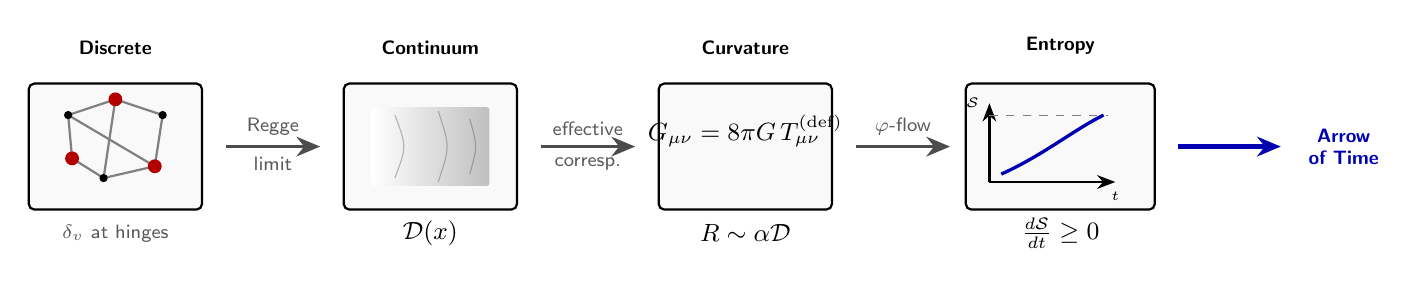
\begin{tikzpicture}[
    box/.style={draw=black, thick, rounded corners=2pt, minimum width=2.2cm, minimum height=1.6cm, align=center, fill=gray!5},
    arrow/.style={-{Stealth[length=3mm, width=2.5mm]}, very thick, black!70},
    sublabel/.style={font=\scriptsize\sffamily, gray!70!black},
    mathlabel/.style={font=\small},
    stage/.style={font=\scriptsize\sffamily\bfseries, above}
]
% STAGE 1: Discrete Complex
\begin{scope}[shift={(0,0)}]
    \node[box] (box1) at (0,0) {};
    \node[stage] at (0,1.05) {Discrete};
    \coordinate (n1) at (-0.6,0.4);
    \coordinate (n2) at (0,0.6);
    \coordinate (n3) at (0.6,0.4);
    \coordinate (n4) at (0.5,-0.25);
    \coordinate (n5) at (-0.15,-0.4);
    \coordinate (n6) at (-0.55,-0.15);
    \draw[gray, thick] (n1)--(n2)--(n3)--(n4)--(n5)--(n6)--(n1);
    \draw[gray, thick] (n2)--(n5); \draw[gray, thick] (n1)--(n4);
    \fill[black] (n1) circle (1.5pt); \fill[black] (n3) circle (1.5pt); \fill[black] (n5) circle (1.5pt);
    \fill[red!70!black] (n2) circle (2.5pt); \fill[red!70!black] (n4) circle (2.5pt); \fill[red!70!black] (n6) circle (2.5pt);
    \node[sublabel] at (0,-1.1) {$\delta_v$ at hinges};
\end{scope}
% Arrow 1->2
\draw[arrow] (1.4,0) -- node[above, sublabel] {Regge} node[below, sublabel] {limit} (2.6,0);
% STAGE 2: Defect Field
\begin{scope}[shift={(4,0)}]
    \node[box] (box2) at (0,0) {};
    \node[stage] at (0,1.05) {Continuum};
    \shade[left color=white, right color=gray!50, rounded corners=1pt] (-0.75,-0.5) rectangle (0.75,0.5);
    \draw[gray!60] (-0.45,-0.4) .. controls (-0.3,0) .. (-0.45,0.4);
    \draw[gray!70] (0.1,-0.45) .. controls (0.25,0) .. (0.1,0.45);
    \draw[gray!80] (0.5,-0.35) .. controls (0.6,0) .. (0.5,0.35);
    \node[mathlabel] at (0,-1.1) {$\Defect(x)$};
\end{scope}
% Arrow 2->3
\draw[arrow] (5.4,0) -- node[above, sublabel] {effective} node[below, sublabel] {corresp.} (6.6,0);
% STAGE 3: Curvature
\begin{scope}[shift={(8,0)}]
    \node[box] (box3) at (0,0) {};
    \node[stage] at (0,1.05) {Curvature};
    \node[font=\small] at (0,0.2) {$G_{\mu\nu} = 8\pi G\, T_{\mu\nu}^{(\text{def})}$};
    \node[mathlabel] at (0,-1.1) {$R \sim \alpha\Defect$};
\end{scope}
% Arrow 3->4
\draw[arrow] (9.4,0) -- node[above, sublabel] {$\varphi$-flow} (10.6,0);
% STAGE 4: Entropy
\begin{scope}[shift={(12,0)}]
    \node[box, minimum width=2.4cm] (box4) at (0,0) {};
    \node[stage] at (0,1.05) {Entropy};
    \draw[-{Stealth}, thick] (-0.9,-0.45) -- (-0.9,0.55) node[left, font=\tiny] {$\Ent$};
    \draw[-{Stealth}, thick] (-0.9,-0.45) -- (0.7,-0.45) node[below, font=\tiny] {$t$};
    \draw[blue!70!black, very thick] (-0.75,-0.35) .. controls (-0.2,-0.1) and (0.15,0.2) .. (0.55,0.4);
    \draw[gray, dashed] (-0.9,0.4) -- (0.6,0.4);
    \node[mathlabel] at (0,-1.1) {$\tfrac{d\Ent}{dt} \geq 0$};
\end{scope}
% Final arrow to "Arrow of Time"
\draw[arrow, blue!70!black, line width=1.5pt] (13.5,0) -- (14.8,0);
\node[font=\scriptsize\sffamily\bfseries, blue!70!black, align=center] at (15.6,0) {Arrow\\of Time};
\end{tikzpicture}
\caption{The discrete-to-continuum pipeline. Discrete defects $\delta_v$ at cell complex hinges are coarse-grained to a continuum field $\Defect(x)$, which sources effective curvature via the field equations. Under $\phigr$-scaled Laplace--Beltrami flow, the configurational entropy $\Ent[\rho]$ increases monotonically, defining the geometric arrow of time.}
\label{fig:pipeline}
\end{figure}

\subsection{Relation to Gravitational Entropy}
\label{subsec:gravitational-entropy}

The connection between geometry and entropy has been explored extensively, notably by Penrose in the context of the Weyl curvature hypothesis \citep{Penrose1979}. Penrose proposed that gravitational entropy is encoded in the Weyl tensor---the trace-free part of the Riemann tensor---and that the arrow of time corresponds to the growth of Weyl curvature.

Our framework is compatible with this perspective but approaches it differently:

\begin{itemize}
\item \textbf{Defect entropy vs.\ Weyl entropy:} In our framework, entropy is associated with the configurational spread of the defect density, not directly with Weyl curvature. However, since defect accumulation generically produces both scalar curvature (Ricci) and shear (Weyl), the two notions are related.

\item \textbf{Monotonicity:} Both approaches predict monotonic increase of a geometric quantity (defect density / configurational entropy in our case, Weyl curvature in Penrose's). The physical mechanisms are distinct but potentially complementary.

\item \textbf{Initial conditions:} Penrose's hypothesis requires a low-Weyl initial state; our framework requires an initial state of (approximate) local closure. These are different but not incompatible conditions.
\end{itemize}

A full reconciliation of these approaches lies beyond the scope of this paper and is left for future work.

A clarification regarding scope is warranted. The framework developed here applies at two scales: (i) the discrete scale, where cell complexes, defects, and graph Laplacians are defined; and (ii) the effective continuum scale, where the Laplace--Beltrami correspondence and Einstein-compatible field equations emerge. Large-scale cosmological dynamics---including the expansion history of the universe, structure formation, and the precise value of the cosmological constant---are \emph{not} derived from this framework. While the observation that uniform defect backgrounds contribute an effective vacuum energy term (Eq.~\ref{eq:defect-cosmological}) is suggestive, it does not constitute a cosmological model. No Friedmann equations are derived, no inflationary mechanism is proposed, and no quantitative cosmological predictions are claimed. The extension of this framework to cosmological scales remains a direction for future work, requiring additional assumptions and constraints not developed here.

% ============================================================
% SECTION 5: PREDICTIONS AND TESTS
% ============================================================
\section{Predictions and Tests}
\label{sec:predictions}

A framework without falsifiable predictions is not scientific. In this section, we present concrete predictions, specify what would falsify them, and outline pathways for testing.

\subsection{Summary of Predictions}

\begin{table}[ht]
\centering
\caption{Falsifiable predictions of the geometric non-closure framework.}
\label{tab:predictions}
\begin{tabular}{@{}p{4cm}p{4cm}p{4cm}@{}}
\toprule
\textbf{Prediction} & \textbf{Expected Signature} & \textbf{Falsification Criterion} \\
\midrule
\textbf{P1:} Defect density correlates with curvature & $\Defect(x) \sim R(x)$ (positive correlation) in regions of positive scalar curvature & Strong negative correlation or no correlation in discrete simulations \\
\addlinespace
\textbf{P2:} $\phigr$-scaling in spectral decay & Contraction rates scale as $\phigr \lambda_k$ for eigenvalue $\lambda_k$ & Contraction rates inconsistent with $\phigr$ to within 5\% \\
\addlinespace
\textbf{P3:} Entropy monotonicity under expansion & $d\Ent/dt \geq 0$ for all expansion protocols & Observation of spontaneous entropy decrease in closed system \\
\addlinespace
\textbf{P4:} Defect accumulation at boundaries & Higher defect density at interfaces of expanding domains & Uniform defect distribution independent of boundary \\
\addlinespace
\textbf{P5:} Effective cosmological constant from uniform defects & $\Lambda_{\text{eff}} \propto \Defect_0^2$ for background defect density & $\Lambda_{\text{eff}}$ uncorrelated with defect measures \\
\addlinespace
\textbf{P6:} Discrete-continuum spectral convergence & Graph Laplacian spectrum converges to Laplace--Beltrami spectrum under refinement & Spectral divergence or non-convergence under refinement \\
\bottomrule
\end{tabular}
\end{table}

\subsection{Discrete Simulation Pathway}

The most direct test of the framework is through discrete simulation. The procedure is:

\begin{enumerate}
\item \textbf{Initialise:} Construct a locally closed cell complex (e.g., the boundary of a 120-cell or a portion thereof).

\item \textbf{Extend:} Iteratively attach new cells according to a specified growth rule, recording defect locations where local closure fails.

\item \textbf{Measure:} Compute the defect density field $\Defect(x)$, the spectral properties of the graph Laplacian, and the configurational entropy.

\item \textbf{Evolve:} Apply $\phigr$-scaled Laplacian dynamics and measure contraction rates.

\item \textbf{Compare:} Verify predictions P1--P6 against simulation data.
\end{enumerate}

Pseudocode for this procedure is provided in Appendix~\ref{app:pseudocode}.

\subsection{Continuum Modelling Pathway}

For continuum tests, the procedure is:

\begin{enumerate}
\item \textbf{Specify geometry:} Choose a Riemannian manifold $(\Mani, g)$ with known curvature.

\item \textbf{Initialise defect field:} Specify an initial defect density $\Defect_0(x)$ consistent with the curvature.

\item \textbf{Evolve:} Solve the $\phigr$-scaled Laplace--Beltrami flow \eqref{eq:phi-flow} numerically.

\item \textbf{Compute entropy:} Track $\Ent[\rho_t]$ and verify monotonicity.

\item \textbf{Extract effective curvature:} From the defect field evolution, compute the predicted curvature response and compare with the input geometry.
\end{enumerate}

\subsection{Condensed-Matter and Network Analogues}

The framework admits analogues in condensed-matter and network systems:

\begin{itemize}
\item \textbf{Crystalline defects:} In crystals, dislocations and disclinations are topological defects that carry curvature. The effective correspondence $\Defect \sim R$ has an analogue in the geometry of defected crystals \citep{Kleinert1989}.

\item \textbf{Network growth:} In growing networks (e.g., the World Wide Web, citation networks), preferential attachment rules lead to degree heterogeneity analogous to defect accumulation. Spectral properties of such networks can be compared with predictions.

\item \textbf{Granular packings:} Disordered packings of grains exhibit geometric frustration analogous to non-closure. Force networks in such systems may exhibit defect-like structures.
\end{itemize}

These analogues provide experimental and observational avenues for testing the framework outside the gravitational context.

% ============================================================
% SECTION 6: DISCUSSION
% ============================================================
\section{Discussion}
\label{sec:discussion}

\subsection{What BP3 Reframes}

This paper reframes the relationship between geometry and gravity. Rather than treating curvature as a fundamental field governed by the Einstein equations, we interpret curvature as an effective response to the geometric constraint that local closure cannot be globally maintained.

This reframing does not contradict General Relativity. The Einstein equations remain valid as effective field equations; the defect contribution \eqref{eq:defect-stress-energy} augments but does not replace the standard gravitational dynamics.

The conceptual shift is from:
\begin{center}
\emph{Curvature $\to$ Gravity $\to$ Dynamics}
\end{center}
to:
\begin{center}
\emph{Local Closure Failure $\to$ Defects $\to$ Curvature $\to$ Effective Gravity.}
\end{center}

\subsection{Why $\phigr$ Appears as a Candidate Scaling}

The golden ratio $\phigr = (1 + \sqrt{5})/2$ appears in this framework as a candidate scaling parameter governing contraction rates and entropy evolution. Its appearance is \emph{not} a claim of mystical significance but rather a consequence of the underlying geometry:

\begin{itemize}
\item $\phigr$ arises in the geometry of regular pentagons and icosahedra, which are the building blocks of the 120-cell.

\item The eigenvalue structure of certain symmetric graphs exhibits $\phigr$-related ratios.

\item As a scaling parameter, $\phigr$ satisfies the self-similarity condition $\phigr^2 = \phigr + 1$, which may relate to the iterative nature of cell complex extension.
\end{itemize}

We treat $\phigr$ as a candidate scaling parameter, to be validated or falsified by comparison with simulation and observation (Prediction P2).

\subsection{Known Limitations}

The framework presented here has several known limitations:

\begin{enumerate}
\item \textbf{No quantum effects:} The entire development is classical. Quantum corrections to the defect dynamics and their relation to quantum gravity are not addressed.

\item \textbf{No matter coupling:} We have not specified how matter fields couple to the defect density. The stress-energy $T_{\mu\nu}^{(\text{matter})}$ in Eq.~\eqref{eq:field-equations} is included formally but not derived from the framework.

\item \textbf{Dimensional specificity:} While the principle of non-closure is dimension-independent, the detailed calculations use 4-dimensional structures. Generalisation to other dimensions requires additional work.

\item \textbf{No cosmological predictions:} We have not derived predictions for large-scale cosmology (expansion history, structure formation). The effective cosmological constant \eqref{eq:defect-cosmological} is suggestive but not quantitatively predictive.

\item \textbf{Parameter freedom:} The effective action contains free parameters ($\beta$, $\gamma$) that are not determined by the framework. These must be fixed by matching to observation.
\end{enumerate}

\subsection{What This Framework Does Not Yet Explain}

Several important phenomena are not addressed:

\begin{itemize}
\item The value of the cosmological constant
\item The hierarchy between gravitational and other forces
\item The origin of matter content
\item Black hole thermodynamics and the information paradox
\item The initial conditions of the universe
\end{itemize}

These are directions for future development, not claims of the current framework.

\subsection{Roadmap to Rigorous Derivation}
\label{subsec:roadmap}

While this paper presents the framework at a conceptual and effective level, the path to fully rigorous derivations is well-defined. The key steps, deferred to technical companion work, are:

\begin{enumerate}
\item \textbf{Discrete geometry:} Define the geometric substrate as a regular cell complex $\mathcal{K}$ with specified combinatorial structure (e.g., 120-cell--derived).

\item \textbf{Defect quantification:} Define defects rigorously as angular deficits (Regge-style) or holonomy deficits around codimension-2 faces, as detailed in Appendix~\ref{app:defect}.

\item \textbf{Discrete curvature:} Use Regge calculus or discrete exterior calculus to assign curvature to hinges (codimension-2 simplices) proportional to angular deficit \citep{Regge1961}.

\item \textbf{Measure convergence:} Establish convergence of normalised defect measures on refining cell complexes to curvature invariants on the limiting manifold, following standard results in discrete differential geometry \citep{Desbrun2005}.

\item \textbf{Continuum action:} Show that the discrete action (sum over hinges) converges to the Einstein--Hilbert action plus defect corrections in the continuum limit.
\end{enumerate}

Each step involves technical machinery that would obscure the conceptual narrative of this paper. The present work establishes \emph{what} must be true; the companion work will establish \emph{that} it is true.

\subsection{Relation to Objective Reduction and Quantum--Gravitational Threshold Models}
\label{subsec:OR-compatibility}

To be explicit: this paper does not model consciousness, does not derive wavefunction collapse, and does not validate or invalidate the Orchestrated Objective Reduction (Orch-OR) hypothesis or related quantum--gravitational threshold models. What BP3 does provide is a geometric origin for gravitational degrees of freedom---specifically, the emergence of effective curvature from defect accumulation. This geometric grounding is \emph{compatible} with frameworks that posit gravitational thresholds for state reduction (e.g., Penrose's objective reduction criterion), in the sense that it supplies a discrete-geometric substrate from which such thresholds might, in principle, be derived. However, no such derivation is attempted here, and compatibility should not be read as confirmation. The relationship between geometric non-closure and quantum state dynamics remains an open question for future investigation.

While the present work focuses on contraction and defect accumulation under geometric extension, the complementary role of expansion as a dual geometric process---and its potential implications for the reversal or redistribution of defect density---is deferred to future investigation.

% ============================================================
% SECTION 7: CONCLUSION
% ============================================================
\section{Conclusion}
\label{sec:conclusion}

This paper has developed a framework in which gravity emerges as the effective curvature response to accumulated geometric defects. The key results are:

\begin{itemize}
\item \textbf{Geometric non-closure is inevitable:} Maximally symmetric local configurations (exemplified by the 120-cell) cannot be globally extended without introducing defects. This is a geometric necessity, not a dynamical assumption.

\item \textbf{Defects relate to curvature:} In an effective continuum description, the defect density field $\Defect(x)$ scales with scalar curvature, providing a candidate discrete-geometric origin for spacetime curvature.

\item \textbf{BP2 results lift to continuum:} The $\phigr$-scaled contraction and entropy monotonicity established in Bridge Paper~2 generalise to Riemannian manifolds via the Laplace--Beltrami correspondence.

\item \textbf{Entropy monotonicity defines the arrow of time:} The irreversible accumulation of defects and the monotonic increase of configurational entropy provide an intrinsic geometric arrow of time.

\item \textbf{Effective field equations are Einstein-compatible:} The variation of the effective action yields field equations of Einstein form, supplemented by defect-induced stress-energy.

\item \textbf{Predictions are falsifiable:} The framework generates specific, testable predictions that can be evaluated through discrete simulation, continuum modelling, and condensed-matter analogues.

\item \textbf{Future development is clearly delineated:} Known limitations and open questions have been identified, providing a roadmap for subsequent work.
\end{itemize}

The framework presented here does not claim to be a final theory. It is offered as a candidate explanatory structure that connects discrete geometry, entropy, and gravity in a unified language. The test of its value lies in the predictions of Section~\ref{sec:predictions} and in the fruitfulness of the research directions it suggests.

% ============================================================
% ACKNOWLEDGEMENTS
% ============================================================
\section*{Acknowledgements}

The author thanks colleagues and correspondents who provided feedback on earlier drafts of this work. This research was conducted under the auspices of the Vibrational Field Dynamics Institute.

% ============================================================
% REFERENCES
% ============================================================
\bibliographystyle{plainnat}
\begin{thebibliography}{99}

\bibitem[BP2(2025)]{BP2}
L.~Smart.
\newblock Bridge Paper 2: $\varphi$-Scaled Contraction and Entropy Monotonicity on Geometric Graphs.
\newblock \textit{Vibrational Field Dynamics Institute}, 2025.

\bibitem[Coxeter(1973)]{Coxeter1973}
H.~S.~M.~Coxeter.
\newblock \textit{Regular Polytopes}.
\newblock Dover Publications, New York, 3rd edition, 1973.

\bibitem[Desbrun et al.(2005)]{Desbrun2005}
M.~Desbrun, E.~Kanso, and Y.~Tong.
\newblock Discrete differential forms for computational modeling.
\newblock In \textit{Discrete Differential Geometry}, Oberwolfach Seminars, pages 287--324. Birkh\"auser, 2005.

\bibitem[Kleinert(1989)]{Kleinert1989}
H.~Kleinert.
\newblock \textit{Gauge Fields in Condensed Matter}.
\newblock World Scientific, Singapore, 1989.

\bibitem[Penrose(1979)]{Penrose1979}
R.~Penrose.
\newblock Singularities and time-asymmetry.
\newblock In S.~W. Hawking and W.~Israel, editors, \textit{General Relativity: An Einstein Centenary Survey}, pages 581--638. Cambridge University Press, 1979.

\bibitem[Regge(1961)]{Regge1961}
T.~Regge.
\newblock General relativity without coordinates.
\newblock \textit{Il Nuovo Cimento}, 19(3):558--571, 1961.

\bibitem[Wald(1984)]{Wald1984}
R.~M.~Wald.
\newblock \textit{General Relativity}.
\newblock University of Chicago Press, 1984.

\end{thebibliography}

% ============================================================
% APPENDICES
% ============================================================
\appendix

\section{Mathematical Assumptions in Discrete-to-Continuum Lift}
\label{app:assumptions}

The lift from discrete graph structures to continuum manifolds relies on the following mathematical assumptions:

\begin{assumption}[Graph Sequence]
There exists a sequence of finite graphs $\{G_n\}_{n=1}^\infty$ with $|V(G_n)| \to \infty$ such that:
\begin{enumerate}[label=(\alph*)]
\item Each $G_n$ is connected and has bounded vertex degree.
\item The graphs $G_n$ are embedded in a fixed compact Riemannian manifold $(\Mani, g)$.
\item The mesh size $h_n \defeq \max_{v \in V(G_n)} \text{dist}(v, \text{nearest neighbour}) \to 0$ as $n \to \infty$.
\end{enumerate}
\end{assumption}

\begin{assumption}[Spectral Convergence]
The eigenvalues $\{\lambda_k^{(n)}\}$ of the normalised graph Laplacian $L_n$ converge to the eigenvalues $\{\lambda_k\}$ of the Laplace--Beltrami operator $\LaplB$ on $(\Mani, g)$:
\[
\lim_{n \to \infty} \lambda_k^{(n)} = \lambda_k \quad \text{for each } k \geq 0.
\]
\end{assumption}

\begin{assumption}[Function Convergence]
For any smooth function $f \in C^\infty(\Mani)$, its restriction to the vertex set $f|_{V(G_n)}$ satisfies:
\[
\lim_{n \to \infty} \sum_{v \in V(G_n)} |L_n f(v) - \LaplB f(v)|^2 \cdot \text{Vol}(v) = 0,
\]
where $\text{Vol}(v)$ is the Voronoi volume associated with vertex $v$.
\end{assumption}

These assumptions are standard in the numerical analysis literature and are satisfied by various graph constructions, including Delaunay triangulations and random geometric graphs under appropriate conditions.

\section{Defect Density Definitions}
\label{app:defect}

We provide several equivalent characterisations of the defect density:

\textbf{Definition (Angular Deficit):}
At a vertex $v$ in a simplicial complex, the angular deficit is
\[
\delta_v = 2\pi - \sum_{\sigma \ni v} \theta_\sigma^{(v)},
\]
where $\theta_\sigma^{(v)}$ is the dihedral angle at $v$ in simplex $\sigma$. In dimension $n$, the appropriate solid angle generalisation is used.

\textbf{Definition (Combinatorial Deficit):}
In a cell complex where each vertex should have valence $k$ (for local closure), the combinatorial deficit at $v$ is
\[
\delta_v^{(\text{comb})} = k - \deg(v),
\]
where $\deg(v)$ is the actual vertex degree.

\textbf{Definition (Holonomy Deficit):}
For a connection on a fibre bundle over the complex, the holonomy around a small loop encircling $v$ defines a group element $g_v$. The deficit is
\[
\delta_v^{(\text{hol})} = \|g_v - e\|,
\]
where $e$ is the identity and $\|\cdot\|$ is an appropriate norm on the group.

In the continuum limit, these definitions coalesce into the defect density $\Defect(x)$ via Eq.~\eqref{eq:defect-density}.

\section{Entropy Monotonicity Conditions}
\label{app:entropy}

The monotonicity of the configurational entropy functional requires the following conditions:

\begin{enumerate}
\item \textbf{Positivity of diffusion coefficient:} The $\phigr$-scaled flow $\partial_t \rho = \phigr \LaplB \rho$ requires $\phigr > 0$, which is satisfied since $\phigr \approx 1.618$.

\item \textbf{Positivity of density:} The entropy $\Ent[\rho] = -\int \rho \log \rho$ is well-defined only for $\rho > 0$ almost everywhere. Under the heat equation, positivity is preserved if $\rho_0 > 0$.

\item \textbf{Completeness of manifold:} The manifold $(\Mani, g)$ must be complete to ensure that the heat kernel exists and has the required properties.

\item \textbf{Lower bound on Ricci curvature:} For entropy monotonicity with precise rates, a lower bound $\text{Ric} \geq -Kg$ for some $K \geq 0$ is typically assumed (Bakry--Émery theory).
\end{enumerate}

Under these conditions, the entropy increase formula \eqref{eq:entropy-increase} holds, with the rate controlled by the spectral gap $\lambda_1^{(\text{LB})}$.

\section{Simulation Pseudocode}
\label{app:pseudocode}

The following pseudocode outlines a discrete simulation of the geometric non-closure framework:

\begin{verbatim}
ALGORITHM: Geometric Non-Closure Simulation

INPUT:
  - Initial cell complex K_0 (e.g., 120-cell boundary)
  - Growth rule G (specifies how to attach new cells)
  - Number of expansion steps N
  - Time evolution steps T
  - Scaling parameter phi = (1 + sqrt(5)) / 2

OUTPUT:
  - Defect density field D
  - Spectral data (eigenvalues, eigenvectors)
  - Entropy trajectory S(t)

PROCEDURE:

1. INITIALISATION
   K <- K_0
   D <- empty array  // defect locations

2. EXPANSION LOOP (cell growth)
   FOR step = 1 TO N:
     boundary <- get_boundary_cells(K)
     FOR each cell c in boundary:
       new_cell <- generate_cell(c, G)
       IF local_closure_fails(K, new_cell):
         record_defect(D, attachment_vertex)
       K <- attach(K, new_cell)
     END FOR
   END FOR

3. CONSTRUCT LAPLACIAN
   V <- vertices(K)
   E <- edges(K)
   L <- graph_laplacian(V, E)  // L = D - A

4. SPECTRAL ANALYSIS
   eigenvalues, eigenvectors <- eigendecompose(L)
   VERIFY: eigenvalues[k] scale as predicted

5. ENTROPY EVOLUTION
   rho_0 <- initial_distribution(V)
   S <- []
   FOR t = 0 TO T:
     rho_t <- evolve(rho_{t-1}, phi * L, dt)
     S[t] <- compute_entropy(rho_t)
   END FOR
   VERIFY: S is non-decreasing

6. DEFECT-CURVATURE CORRELATION
   D_field <- interpolate_defect_density(D, V)
   R_field <- estimate_scalar_curvature(K)
   correlation <- compute_correlation(D_field, R_field)
   VERIFY: correlation > 0 (Prediction P1)

7. RETURN D, eigenvalues, S

HELPER FUNCTIONS:

local_closure_fails(K, new_cell):
  // Check if attaching new_cell violates local closure
  v <- attachment_vertex(new_cell)
  link <- vertex_link(K, v)
  RETURN NOT is_closed_manifold(link)

compute_entropy(rho):
  S <- 0
  FOR each v in V:
    IF rho[v] > 0:
      S <- S - rho[v] * log(rho[v])
  RETURN S

evolve(rho, L_scaled, dt):
  // One step of heat equation: d rho / dt = L_scaled * rho
  RETURN rho + dt * L_scaled @ rho
\end{verbatim}

\section{Notation Table}
\label{app:notation}

\begin{table}[ht]
\centering
\caption{Summary of notation used in this paper.}
\begin{tabular}{@{}ll@{}}
\toprule
\textbf{Symbol} & \textbf{Meaning} \\
\midrule
$\phigr$ & Golden ratio, $\phigr = (1 + \sqrt{5})/2 \approx 1.618$ \\
$\mathcal{K}$ & Cell complex \\
$\mathcal{K}^{(k)}$ & Set of $k$-cells in $\mathcal{K}$ \\
$V$, $E$ & Vertex set, edge set of a graph \\
$L$ & Graph Laplacian, $L = D - A$ \\
$\LaplB$ & Laplace--Beltrami operator on $(\Mani, g)$ \\
$\Defect(x)$ & Defect density field \\
$\delta_v$ & Angular/combinatorial deficit at vertex $v$ \\
$\Ent[\rho]$ & Configurational entropy functional \\
$\rho$ & Probability density / distribution \\
$(\Mani, g)$ & Riemannian manifold with metric $g$ \\
$R$ & Scalar curvature \\
$R_{\mu\nu}$ & Ricci tensor \\
$G_{\mu\nu}$ & Einstein tensor, $G_{\mu\nu} = R_{\mu\nu} - \frac{1}{2}Rg_{\mu\nu}$ \\
$T_{\mu\nu}$ & Stress-energy tensor \\
$\Lambda$ & Cosmological constant \\
$G$ & Newton's gravitational constant \\
$\alpha, \beta, \gamma$ & Coupling constants in effective action \\
$\lambda_k$ & $k$-th eigenvalue of Laplacian \\
$\lambda_1$ & Spectral gap (first nonzero eigenvalue) \\
\bottomrule
\end{tabular}
\end{table}

% ============================================================
% END DOCUMENT
% ============================================================
\end{document}
